% !TeX root = 00_nesting_paper.tex
\subsection{Two HOp Separated Patterns Algorithm}\label{sec:THOSPA}
We now want to focus on a specific instance of the problem stated in Algorithm \ref{alg:general}: suppose to store a graph using adjacency lists \texttt{[similarly to the one proposed in the Graph Join algorithm]}; in particular, the previous data structure is now extended with both vertex and edge containment, plus with both ingoing and outgoing edges for each single graph vertex. The latter requirement is added in order to satisfy the possibility to visit the edges backwards, thus allowing to navigate the graph in each possible direction. The main data structure over which this algorithm relies  is presented in Figure \ref{nestedGraphVertex}: it shows that minor changes have been applied to the original data structure that was used to serialize graph within the graph join scenario. %Moreover, in this case we mark with different hash values the vertices within the data structure satisfying different predicates within the predicates. 
Given that the data structure requires a simple linear visit of the graph, no additional primary and secondary data structures are required. Nevertheless, during our serialization phase we provide both a primary index for accessing external informations (\textit{VertexIndex}) and the serialization of all the vertices' adjacency lists, which is going to be used for traversing the graph (\textit{VertexVals}). In our straightforward implementation, hash values are here used only as placeholders for the nodes' labels used within the patterns but, given that vertices are not sorted by hash value as for graph joins, we keep the hash fields for both backward compatibility and in order to make graph joins possible for nested graphs, too.


Let us now restrict $\alpha$ to one single vertex and two edges: for each vertex $v$ matched by $\alpha$ ($\alpha\vDash v$) we know that we must (possibly) visit all the edges going from $v$ towards the vertices $\gamma_E^{src}$ and $\gamma_E^{dst}$, that substantially are $\gamma_V$. Please note that if in $g_E$ there is no path connecting $\alpha$ to $\gamma_E^{src}$ or $\gamma_E^{dst}$, the problem may quickly become cubic with respect to the size of the vertices, because we must create all the possible permutations where $v$ is present alongside another element matching $\gamma_E^{src}$ or $\gamma_E^{dst}$. Therefore, having an edge as a constraint in $\alpha$ linking $v$ towards $\gamma_E^{src}$ or $\gamma_E^{dst}$ both in $g_E$ and $g_V$ can reduce all the possible computations to the actual edges traversed from $v$ meeting the grouping references. Therefore, we know whether we finished visiting our patterns after exhaustively matching all the elements within the pattern. We can now reduce the cost to check when we finished traversing all the elements reaching  $\gamma_E^{src}$ and $\gamma_E^{dst}$ from $v$  after a linear scan of all the ingoing or outgoing nodes. Hereby, the most simple graph nesting example is where $v$ is the middle node between a path between $\gamma_E^{src}$ and $\gamma_E^{dst}$ vertices. 

\begin{figure*}
	\centering
	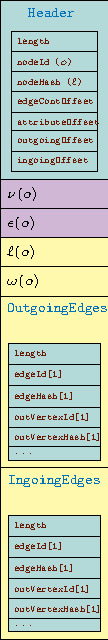
\includegraphics[height=.7\textheight,angle =90]{/mnt/DEC4763AC47614CD/thesis/imgs/10nesting/test}
	\caption{Extending the serialized graph data structure presented for graph join for the nesting operation. In particular, the present data structure extends each vertex representation in $VertexVals$ (Figure \ref{fig:graphstructure}) in order to fully supports the nested graph data model:
		entities and relationships may now be contained into another data node (either a vertex or an edge). The first block of the serialized data structure contains the pointers towards the memory regions containing data which may vary in size. The fuchsia nodes remark the memory spaces where such data containments may be stored. Moreover, ingoing edges are stored as well as outgoing edges. }\label{nestedGraphVertex}
\end{figure*}
\begin{algorithm}[!t]
	\caption{Two HOp Separated Patterns Algorithm (THoSP)}\label{alg:THoSPAlgorithm}
	\begin{adjustbox}{max width=\textwidth}
		\begin{minipage}{1.2\linewidth}
			\algrenewcommand\algorithmicindent{1em}
			\begin{algorithmic}[1]
				\Procedure{PartitionHashJoin}{$(g_V,\gamma_V),({g_E},\gamma_E^{src},\gamma_E^{dst});\; \nested$}
				\State \textsc{File} $AdjFile$ = \textsc{Open}($\nested$);
				\State \textsc{File} $Nesting$ = \textsc{Open}(\textbf{new});
				\State \textsc{Adjacency} $toSerialize$ = \par \textbf{new} \textsc{Map<Vertex,<Edge,Vertex>>}();
				\State {$\alpha:=g_V\cap {g_E}\backslash(\gamma_V\cup\gamma_E)$;}
				\For{\textbf{each vertex} $v$ in $AdjFile$}
				\If{$\alpha\vDash v$} 
				\For {\textbf{each} $\gamma_V\vDash (u,e,v)$} 
				\State{$u':=dt(1,dt(0,u))$} 
				\State{$NestingIndex$.write($\Braket{u',u}$)} 
				\State{$NestingIndex$.write($\Braket{u',e}$)}
				\State{$NestingIndex$.write($\Braket{u',v}$)}
				\If{$\gamma_E\vDash (v,e,u,e',w)$}
				\State{$w':=dt(1,dt(0,w))$} 
				\State{$\varepsilon:=dt(1,dt(u,w))$}
				\State{$NestingIndex$.write($\Braket{\varepsilon,u}$)}
				\State{$NestingIndex$.write($\Braket{\varepsilon,e}$)}
				\State{$NestingIndex$.write($\Braket{\varepsilon,w}$)}
				\State{$NestingIndex$.write($\Braket{\varepsilon,e'}$)}
				\State{$NestingIndex$.write($\Braket{\varepsilon,v}$)} 
				\State{$toSerialize$.put($u'$,$\Braket{\varepsilon,w'}$)}
				\EndIf
				\EndFor
				\EndIf
				\EndFor
				$AdjFile$.serialize($toSerialize$);
				
				\EndProcedure
			\end{algorithmic}
		\end{minipage}
	\end{adjustbox}
\end{algorithm}
\begin{table*}[!t]
	\centering
	\begin{tabular}{@{}cr|rr@{}}
		\toprule
		{\textbf{Operands' Vertices}} & Matched Graphs  & {\textbf{General Nesting} (ms)} & {\textbf{THoSP} (ms)}  \\	
		\midrule
		$10$ & $3$ &  0.57       & 0.11\\
		$10^2$ & $58$  & 0.73        & 0.14\\
		$10^3$  & $968$  & 2.78   & 0.46\\
		$10^4$ & $8,683$   & 152.11   & 4.07\\
		$10^5$ & $88,885$   & 14,015.00 & 43.81 \\
		$10^6$  & $902,020$  &  1,579,190.00      & 563.02\\
		$10^7$ & $8,991,417$   &  $>$1H      & 8,202.93\\
		$10^8$ & $89,146,891$   &  $>$1H      & 91,834.20\\
		\bottomrule
	\end{tabular}
	%\end{minipage}
	\caption{Comparing the performances of the THoSP algorithm with the naive General Nesting algorithm. This comparison shows that the previously defined algorithm has a worse performance than the THoSP one. }
	\label{tab:comparisonTwo}
\end{table*}


%The main data structure over which this algorithm relies  is presented in Figure \ref{nestedGraphVertex}: it shows that minor changes have been applied to the original data structure that was used to serialize graph within the graph join scenario. %%Moreover, in this case we mark with different hash values the vertices within the data structure satisfying different predicates within the predicates. 
%Given that the data structure requires a simple linear visit of the graph, no additional primary and secondary data structures are required. Nevertheless, during our serialization phase we provide both a primary index for accessing external informations (\textit{VertexIndex}) and the serialization of all the vertices' adjacency lists, which is going to be used for traversing the graph (\textit{VertexVals}). In our straightforward implementation, hash values are here used only as placeholders for the nodes' labels used within the patterns but, given that vertices are not sorted by hash value as for graph joins, we keep the hash fields for both backward compatibility and in order to make graph joins possible for nested graphs, too.

Finally, Algorithm \ref{alg:THoSPAlgorithm} provides the desired implementation of the THoSP algorithm: we can observe that THoSP does not include the data serialization preprocessing step because the data indexing provided at that step is not required by the present algorithm. The main memory is used to create the graph (represented as an adjacency list) that is going to be later on serialized using the same data structure used for providing the result for graph joins, that is an adjacency list where only the vertices' and edges' id appear. This choice is also done both for backward compatibility with respect to the graph join data structure \cite{bergamimm17} and for representing the nesting containment as a separate data structure. We can easily observe that this approach may slow down the whole algorithm, that can be quickened by directly storing the graph representation in secondary memory by using linear hashing. The nesting data structure is stored in a $NestingIndex$ file as a set of pairs $\Braket{u,v}$, where $u$ represents the containing object and $v$ represents the content. By doing so, we omit the \texttt{Group By} cost which affects the previously seen query languages, thus allowing to an overall better performance. Even in this case, a join is performed between the two nested patterns: this is evident from the two nested for loops appearing in the algorithm. 

Table \ref{tab:comparisonTwo} provides a comparison between the general Nesting Algorithm \texttt{[Should we put the previous CIKM version on arXive, so that here we just focus on the main\\ algorithm?]} and over the THoSP implementation of the query provided in our running example, under the assumptions that are going to be soon introduced in the next section. In particular, while THoSP increases linearly alongside the data size, the general nesting algorithm grows quadratically, thus quickly leading to a intractable time evaluation for big data scenarios. Hereby, the THoSP algorithm is going to be used in comparisons with other problem-specific queries on different query languages and data structures.